\documentclass{article}

% Language setting
% Replace `english' with e.g. `spanish' to change the document language
\usepackage[portuguese]{babel}

% Set page size and margins
% Replace `letterpaper' with `a4paper' for UK/EU standard size
\usepackage[letterpaper,top=3cm,bottom=2cm,left=3cm,right=2cm,marginparwidth=1.75cm]{geometry}

% Useful packages
\usepackage{amsmath}
\usepackage{graphicx}
\usepackage[colorlinks=true, allcolors=blue]{hyperref}

\title{Relatório do EP de MAC0209}
\author{
    Antonio Fernando Silva e Cruz Filho\\
    Cássio Azevedo Cancio\\
    Eduardo Mendes Lopes\\
    Guilherme Mota Pereira\\
    Larissa Vitoria Medeiros Silva\\
    Luiz Gabriel Lima Arrais
}

\begin{document}
\maketitle


\begin{abstract}
Esse exercício-programa foi feito para a matéria de Modelagem e Simulação. O trabalho foi dividido em duas partes: na primeira, o objetivo era utilizar uma plataforma de coleta de imagens de ruas e rodovias, Kartaview, para fazer a análise de diferentes métodos de medição de distância e compará-los. Na segunda parte, foi necessário fazer a modelagem de diferentes movimentos. O grupo escolheu analisar o Bloco na Rampa e o Movimento Circular.
\end{abstract}

\newpage

\tableofcontents

\newpage

\section{Cronograma}

\subsection{Gantt Chart}

\begin{center}
\frame{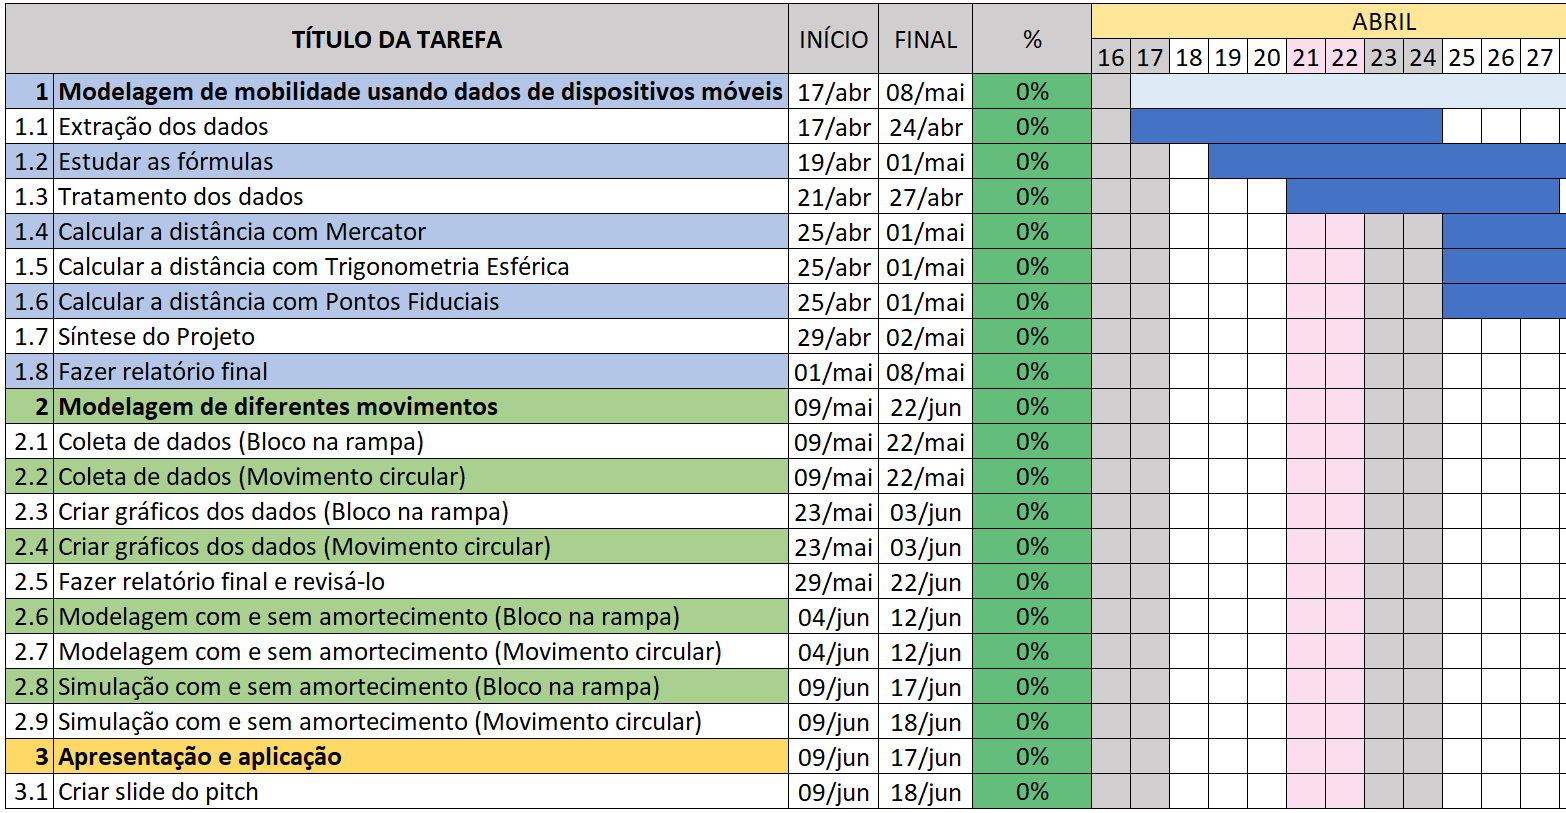
\includegraphics[width=13cm]{./img/Parte 1.png}}\\
\frame{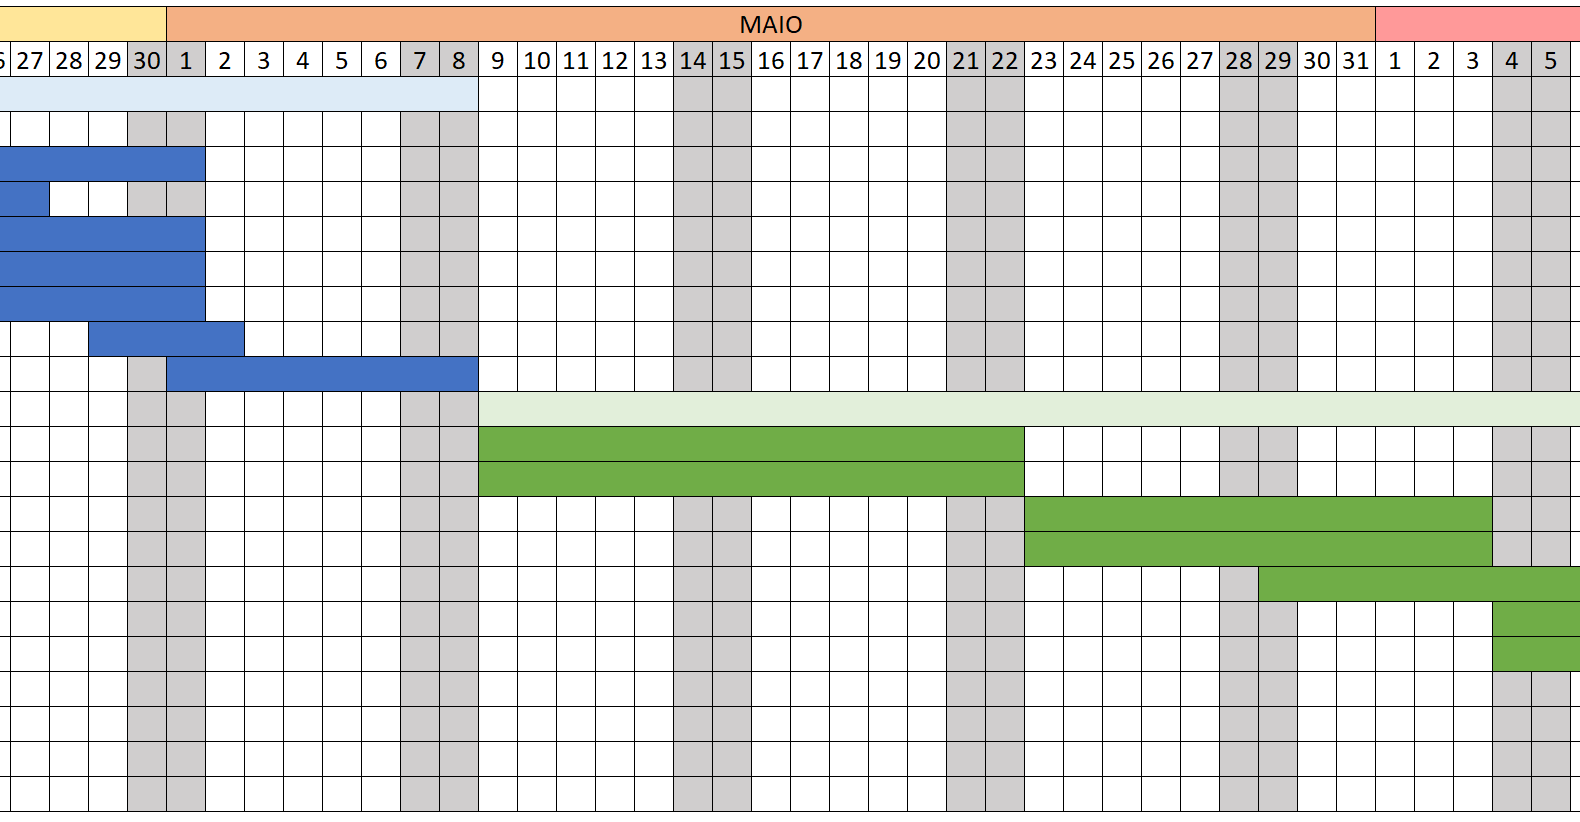
\includegraphics[width=13cm]{./img/Parte 2.png}}\\
\frame{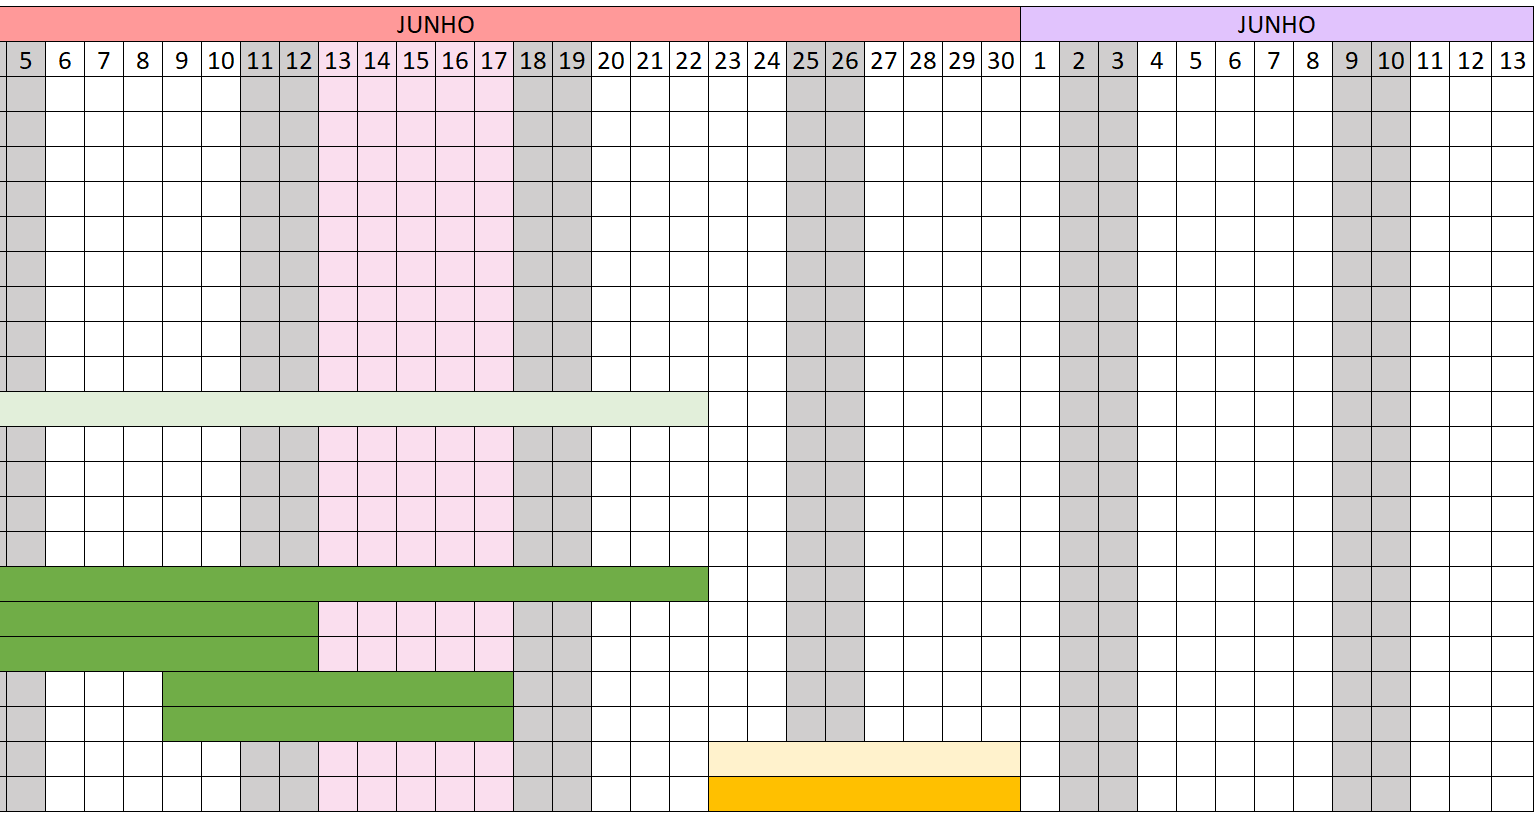
\includegraphics[width=13cm]{./img/Parte 3.png}}
\end{center}

\section{Kartaview (máximo de 4 páginas)}

\subsection{Introdução}

Primeiramente, foi necessário escolher duas rodovias, uma no Brasil e outra no exterior, para que os métodos de desenvolvidos pudessem ser testados. Basicamente, o Kartaview disponibiliza fotos retiradas por um celular em algum trajeto percorrido por um usuário da plataforma de carro. O grupo decidiu utilizar um trecho da rodovia SP-248 próximo à cidade do Guarujá, em São Paulo, já o trecho no exterior, foi a rodovia M6 no Reino Unido, próximo à vila de Old Hutton em South Lakeland.

\subsection{Objetivos}

Apresente o objetivo dessa parte do trabalho. Seja {\bf objetivo e claro}.

\subsection{Dados e métodos}

Explique os dados usados e os métodos desenvolvidos.

\subsection{Resultados experimentais}

Apresente os resultados obtidos, Explore tabelas e gráficos ilustrativos.

\subsection{Discussão}

Interprete os resultados e apresente uma visão crítica.

\newpage

\section{Modelos de movimentos diversos (máximo de 4 páginas)}

\subsection{Introdução}

Apresente uma introdução ao trabalho desenvolvido, fornecendo o contexto e a motivação.

\subsection{Objetivos}

Apresente o objetivo dessa parte do trabalho. Seja {\bf objetivo e claro}.

\subsection{Dados e métodos}

Explique os dados usados e os métodos desenvolvidos.

\subsection{Resultados experimentais}

Apresente os resultados obtidos, Explore tabelas e gráficos ilustrativos.

\subsection{Discussão}

Interprete os resultados e apresente uma visão crítica.

\newpage

\section{Aplicação (máximo de 4 páginas)}

\subsection{Introdução}

Apresente uma introdução ao trabalho desenvolvido, fornecendo o contexto e a motivação.

\subsection{Objetivos}

Apresente o objetivo dessa parte do trabalho. Seja {\bf objetivo e claro}.

\subsection{Dados e métodos}

Explique os dados usados e os métodos desenvolvidos.

\subsection{Resultados experimentais}

Apresente os resultados obtidos, Explore tabelas e gráficos ilustrativos.

\subsection{Discussão}

Interprete os resultados e apresente uma visão crítica.

\end{document}